\documentclass{/home/daniel/GitHub/CITIUS/Apuntes/Template}
\addbibresource{Blibiografia.bib} % si quieres incluir la bibliografía

% Portada 
\title{\Huge \textbf{Introducción a las FPGAs}}
\author{\Large Daniel Vázquez Lago}

% Documento
\begin{document}
\pagenumbering{Roman}
\maketitle
\tableofcontents
\pagenumbering{arabic}
\setlength{\parskip}{2.2mm} % Cambia el espacio entre párrafos

\chapter{Sistemas FPGA}

\section{Concepctos básicos}

En esta sección introduciremos los conceptos básicos en diseño lógico. Presentaremos terminología importante usada en el resto del libro.

\subsection{Álgebra Booleana}

El \textbf{álgebra Booleana} representa las funciones lógicas de los circuitos digitales. Cualquier red de interruptores puede ser modelado por funciones Booleanas. Usamos el álgebra Booleana para describir \textbf{funciones lógicas combinacionales}. Las funciones lógicas básicamente permiten transformar una serie de \textit{inputs} (parámetros de entrada) en una serie de \textit{ouputs} (parámetros de salida). Sean $a$ y $b$ nuestras variables, definimos las siguientes funciones lógicas. Las funciones elementales (NOT, AND y OR) no tienen definición al ser precismante elementales, mientras que las no elementales las podemos definir a partir de las primeras. Sean $a$ y $b$ dos variables cualquiera, escribimos las funciones lógicas en la \cref{Tab:01-Funciones_Logicas}. 

\begin{table}[H] \centering
    \begin{tabular}{cccc} 
        \toprule 
        \textbf{Nombre} & \textbf{Símbolo } & \textbf{Definición} & \textbf{Ejemplo} \\ \midrule
        NOT & ' &  & (1)'=0 \ (0)'=1 \\
        AND  & $\cdot$ &  & 0$\cdot$0=1; 1$\cdot$0=0; 1$\cdot$1=1  \\
        NAND & |  & a | b = (a$\cdot$b)' & 0|0=1; 1|0 = 1; 1|1=0 \\
        OR  & $+$ &  & 0+0=0; 1+0 = 1; 1+1=1 \\
        NOR & NOR &  a NOR b = (a$+$b)' & 0 NOR 0 = 1; 1 NOR 0 = 0; 1 NOR 1 = 0 \\
        XOR & $\oplus$ & a $\oplus$ b = ab'+a'b & 0 $\oplus$ 0 = 0; 1 $\oplus$ 0 = 1; 1 $\oplus$ 1 = 0\\
        XNOR & XNOR & a XNOR b = (a $\oplus$ b)'  & 0 XNOR 0 = 1; 1 XNOR 0 = 0; \\ \bottomrule
    \end{tabular} 
    \caption{}
    \label{Tab:01-Funciones_Logicas}
\end{table}

Lógicamente, como toda álgebra, el álgebra de Boole sigue ciertas reglas de aritmética básicas, tales como: 

\begin{itemize}
    \item \textbf{Ley asociativa:} a + (b+c) = (a+b)+c; a $\cdot$ (b$\cdot$c) = (a $\cdot$ b )$\cdot$c.
    \item \textbf{Ley distributiva:} (a+b)' = a' $\cdot$ b'; (a$\cdot$b)' = a' $+$ b'
\end{itemize}

\subsection{Símobolos lógicos y eléctricos}

Los símbolos eléctricos más usados son: 

\begin{figure}[H] \centering
\begin{circuitikz}
  % NMOS
  \draw (0,0) node[nmos] (N) {};
  \node[below=0.2cm of N] {n-mosfet};

  % PMOS, desplazado
  \draw (3,0) node[pmos] (P) {};
  \node[below=0.2cm of P] {p-mosfet};

  % Dibuja una resistencia con etiquetas
  \draw (4.5,0) to[R, l=$ $] (7,0);
  
  \node (R) at (6,0) {};
  \node[below=0.8cm of R] {Resistencia};

  % Dibuja un capacitor 
  \draw (8,0) to[C, l=$ $] (10,0);
  \node (C) at (9,0) {};
  \node[below=0.8cm of C] {Capacitor};
\end{circuitikz}
\caption{Símbolos para esquemas eléctricos.}
\end{figure}

Mientras que los símbolos en circuitos lógicos son: 

\begin{figure}[H] \centering
\begin{tikzpicture}[scale=10]

  % Inverter
  \node[not gate US, draw, logic gate inputs=nn] (inv) {};
  \node[below=0.2cm of inv] {NOT};

  % NAND
  \node[nand gate US, draw, logic gate inputs=nn, right=1.5cm of inv] (nand) {};
  \node[below=0.2cm of nand] {NAND};

  % NOR
  \node[nor gate US, draw, logic gate inputs=nn, right=1.5cm of nand] (nor) {};
  \node[below=0.2cm of nor] {NOR};

  % AND
  \node[and gate US, draw, logic gate inputs=nn, below=1.5cm of inv, xshift=0.9 cm]  (and) {};
  \node[below=0.2cm of and] {AND};

  % OR
  \node[or gate US, draw, logic gate inputs=nn, right=1.5cm of and] (or) {};m.
  \node[below=0.2cm of or] {OR};

  % XOR
  \node[xor gate US, draw, logic gate inputs=nn, below=1.5cm of and] (xor) {};
  \node[below=0.2cm of xor] {XOR};

  % XNOR
  \node[xnor gate US, draw, logic gate inputs=nn, right=1.5cm of xor] (xnor) {};
  \node[below=0.2cm of xnor] {XNOR};

\end{tikzpicture}
\caption{Símbolos para esquemas lógicos.}
\end{figure}

\section{Diseño digital y FPGAs}

\subsection{El papel de las FPGAs}

Los \textbf{FPGAs} (\textit{Field Programmable Gate Arrays}, en español matriz de puertas lógicas programable en campo) llenan una necesidad existente en el diseño de sistemas digitales, complementario al rol que juegan los microprocesadores. Los microprocesadores pueden ser usados en una cantidad de entornos enorme, pero porque ellos confian en el software para implementar funciones, aunque son generalmente más lentos y consumen más potencia que los chips diseñados con un único propósito (\textit{customizados}). De manera similar, los FPGAS no son chips a medida, por lo que no son tan buenos en funciones particulares. Sin embargo poseen grandes ventajas: 

\begin{itemize}
    \item No tienes porque esperar a acabar el diseño para obtener un chip funcional: el diseño puede ser programado y testeado inmediantemente. 
    \item Son excelentes prototipos. Cuando un FPGA tiene un diseño final, crear un producto o un chip customizado suele ser mucho más fácil.
    \item El mismo FPGA puede ser usado con diferentes diseños. 
\end{itemize}

El área ocupada por las FPGA ha crecido enormemente en los últimos veinte años desde su introducción. Los \textbf{dispositivos de lógica programable PLD} (\textit{Programmable Logic Devices}) estaban en el mercado desde principios de la década de 1970. Estos dispositivos utilizaban estructuras de lógica de dos niveles para implementar la lógica programada. El primer nivel de lógica, el plano AND, generalmente era fijo, mientras que el segundo nivel, conocido como el plano OR, era programable. Los PLD se programaban, en general, mediante antifuses, que se activaban aplicando altos voltajes para establecer las conexiones.

Se utilizaban con mayor frecuencia como \textbf{lógica de enlace } (\textit{glue logic}): lógica necesaria para interconectar los componentes principales del sistema. A menudo se empleaban en prototipos porque podían programarse e insertarse en una placa en cuestión de minutos, pero no siempre llegaban a formar parte del producto final. Los dispositivos de lógica programable no solían considerarse componentes principales de los sistemas en los que se utilizaban. A medida que los sistemas digitales se hicieron más complejos, se necesitaba lógica programable de mayor densidad, y se hicieron evidentes las limitaciones de la lógica de dos niveles de los PLD. La lógica de dos niveles es útil para funciones lógicas relativamente pequeñas, pero con el aumento del nivel de integración, las estructuras de dos niveles se volvieron demasiado ineficientes.

Las FPGA proporcionaron lógica programable usando lógica multinivel de profundidad arbitraria. Utilizaban tanto elementos de lógica programable como interconexiones programables para construir funciones lógicas multinivel. 

A Ross Freeman se le atribuye generalmente la invención de la FPGA. Su FPGA incluía tanto elementos lógicos programables como una estructura de interconexión programable. Su FPGA también se programaba usando memoria SRAM, no antifuses. Esto permitía fabricar la FPGA utilizando procesos estándar de fabricación VLSI, lo que reducía los costos y ofrecía más opciones de manufactura. También permitía que la FPGA se reprogramara mientras estaba en el circuito; esta era una característica particularmente interesante dado que la memoria flash aún no se utilizaba de forma generalizada.

Xilinx y Altera comercializaron las primeras FPGA basadas en SRAM. Una arquitectura alternativa fue introducida por Actel, que empleaba una arquitectura de antifuses. Esta arquitectura no era reprogramable en el campo, lo que se consideraba una ventaja en situaciones que no requerían reconfiguración. Las FPGA de Actel utilizaban una estructura lógica basada en multiplexores organizada en torno a canales de cableado

Durante muchos años las FPGAs han sido vistos como dispositivos de lógica de enlace y como dispositivos para generar prototipos. Hoy en día son usados en todo tipo de sistemas digitales, especialmente en los siguientes campos:
\begin{itemize}
    \item En sistemas de telecomunicaciones extremadamente rápidos.
    \item Como aceleradores de video en grabadoras de video personales.
\end{itemize}

\subsection{Tipos de FPGA}

Pese a qeu hemos hablado de ellos, aún no hemos definido que es un FPGA. Una buena definición podría ser directamente enumerar las características de los PLDs  y los chips customizado, tales como:

\begin{itemize}
    \item Son partes estándar. No estan diseñadas con un propósito particular, pero si son programadas para un propósito particular.
    \item Implementan lógica multi-nivel. Los bloques lógicos dentro de las FPGAs pueden funcioanr como redes de una profundidad arbitaria. Los PLDs por otro lado solo usan dos niveles lógicos: NAND/NOR, lo que limita el tipo de funciones que se pueden implementar eficientemente, pues cualquier función booleana compleja debe transformarse a una forma de solo dos niveles, lo que puede requerir muchas puertas y dificultar el diseño. 
\end{itemize}
Dad que los FPGAs implementan lógica multinivel, son  a la vez bloques lógicos programables y interconexiones programables. 

Para que una FPGA funcione como un circuito digital personalizado, no basta con tener bloques lógicos programables (por ejemplo, LUTs, flip-flops, multiplexores configurables, etc.); también se necesita un sistema que permita conectarlos de cualquier forma necesaria, lo cual se logra con las interconexiones programables.

\begin{itemize}
    \item Los bloques lógicos programables implementan las operaciones lógicas básicas y permiten que el usuario defina qué función booleana realiza cada bloque.

    \item Las interconexiones programables son una red de caminos (switches, multiplexores, etc.) que permiten unir las entradas y salidas de los bloques lógicos según el diseño que el usuario desee. Gracias a ellas, se puede construir cualquier topología de circuito, desde simples puertas combinacionales hasta máquinas de estado complejas.
\end{itemize}
La combinación de bloques lógicos programables y interconexiones programables se llama \textit{fabric} o \textbf{malla} porque posee una estructura regular que puede ser utilizada eficientemente por las herramientas de diseño que asignan la lógica deseada a la FPGA.

Se utilizan diversas tecnologías para programar las FPGA. Algunas FPGA se programan de forma permanente; otras pueden reprogramarse. Las FPGA reprogramables también se conocen como dispositivos reconfigurables. Las FPGA reconfigurables suelen ser preferidas en la construcción de prototipos porque no es necesario desechar el dispositivo cada vez que se realiza un cambio. Los sistemas reconfigurables también pueden reprogramarse dinámicamente durante el funcionamiento del sistema. Esto permite que un mismo hardware desempeñe varias funciones diferentes. Por supuesto, esas funciones no pueden ejecutarse al mismo tiempo, pero la reconfigurabilidad puede ser muy útil cuando un sistema opera en diferentes modos. Por ejemplo, la pantalla del ordenador Radius funcionaba tanto en modo horizontal (paisaje) como en modo vertical (retrato). Cuando el usuario rotaba la pantalla, un interruptor de mercurio provocaba que la FPGA que gestionaba la pantalla se reprogramara para el nuevo modo.

%El FPGA guarda un diseño como un “mapa” de cómo deben estar los switches, y al aplicarlo físicamente, transforma el chip genérico en un circuito específico que implementa tu lógica de manera real y operativa. Un FPGA no es solo una red de switches y LUTs: es un sistema completo de bloques lógicos, memorias, DSPs, interconexiones, interfaces de E/S y circuitería de gestión, todo integrable y configurable para implementar desde una simple puerta lógica hasta sistemas complejos como microcontroladores, procesadores, o procesadores de señal digital.




\chapter{Tecnología VLSI}

Mientras que el diseño tradicional de los sistemas VLSI (Very Large Scale Integration) tiene sus días contados, el diseño a través de las FPGAs está en auge. Sin embargo, los diseñadores de grandes sistemas FPGA necesitan entender los fundamentos de VLSI para sacar el máximo rendimiento a los FPGAs. La arquitectura de los FPGAs está determinada completamente por las restricciones que imponen los VLSI: estructuras de elementos lógicos, estructuras de interconexión programables, redes de interconexión, configuración, distribución de pines. Entender como las características de los dispositivos VLSI afectan a las estructura FPGA pemitirá al diseñador entender cuales son las mayores ventajas de los FPGAs y minimizar la influencia de sus limitaciones. 

Tomemos por ejemplo las redes de interconexión en FPGAs. La mayor parte de los FPGAs modernos proveen a los diseñadores de diferentes tipos de conexiones: locales, globales... ¿Por qué existen tantos tipos de conexiones? Porque las conexiones son cada vez más dificiles de manejar, debido al aumento de longitud. Entender como funcionan estas diferentes tipos de conexión ayudarán al diseñador a elegir que tipo particular de conexión lógica usar, disminuyendo costes y/o aumentando la eficiencia. 

En este capítulo nos centtaremos en entender los VLSI: fabricación, circuiteria, interconexiones... 

\section{Procesos de manufactura}

\section{Características de los transistores}

\section{Puertas Lógicas CMOS}

En esta sección vamos aprender sobre la lógica CMOS, el elemento baśico en el diseño lógico. Para entender el funcionaiento básico de las puertas lógicas, también debeos entender las características básicas de los transistores. Primero introduciremos el diseño básico de las puertas, dado que las puertas más simples pueden ser entendidas pensando en los transistores como interruptores. 

\subsection{Puertas estáticas complementarias}

Consideremos por el momento los transistores como interruptores perfectos. La condición de encendido será diferente cuando consideremos un transistor tipo P y tipo N: un tipo N está encendido cuando el voltaje de puerta es positivo respecto el sustrato, mientras que en el tipo P estará encendido cuando sea negativo. 

La estructura básica de una puerta CMOS está basa en las \textbf{puertas estáticas complementarias}. ¿Por qué se llaman así? El término estático viene de que la salida se mantiene estable (0 o 1) mientras la entrada no cambie. No requiere un reloj ni refresco para mantener su valor. El término complementario viene de que la red NMOS y la red PMOS son complementarias entre sí, i.e. que alguna de las salidas de los transistores NMOS y PMOS debe estar conectada a la salida en todo momento. 

Está divida en la \textbf{\textit{red pullup}} y \textbf{\textit{red pulldown}}, hechas de transistores tipo-p y tipo-n. La salida de la puerta puede ser conectadas al potencial $V_{DD}$ (\textit{Voltaje Drain to Drain}, normalmente 5 V o el 1 lógico) o al potencial $V_{SS}$ (\textit{Voltaje Source to Source}, normalmente 0 V o el 0 lógico). Las dos redes deben ser complementarias para que podamos obtener una salida no indeterminada, y para que además no exista ningún caso de que la salida esté conectada a ambas a la vez. Veamos algunos ejemplos. 

\subsubsection{Esquema para inversor}

\begin{minipage}{0.65\linewidth}
El esquema para el inversor es extremadamente sencillo pero extremadamente ilustrativo. En este caso la entrada $a$, que puede tener un valor de 1 (volatje 5 V, +) o un valor de 0 (voltaje 0 V, triangular) se conecta a la base del transistor NMOS y PMOS. Como hemos dicho, estos funcionan como interruptores perfectos, pero complementarios. El detector NMOS (abajo) dejará estará encedido (deja pasar corriente) cuando reciba un voltaje positivo (respecto la entrada), es decir, cuando reciba un \textit{input} 1, mientras que el PMOS (arriba) cuando recibe un voltaje negativo (\textit{input} 0). Dado que el NMos está conectado con el $V_{SS}$ (\textit{output} 0), cuando reciba el 1 saldrá el \textit{output} 0, e viceversa cuando se conecte el PMos. 
\end{minipage}
\hfill
\begin{minipage}{0.32\linewidth} \centering
    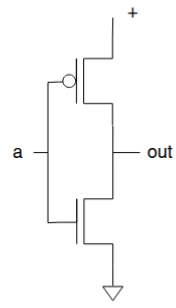
\includegraphics[width=0.5\linewidth]{Imagenes/02-Inversor.png}
    \captionof{figure}{Esquema del inversor con nMOS y pMOS.}
    \label{Fig:02-Inversora}
\end{minipage}

\subsection{Retardo de la Puerta Lógica}

El \textbf{retardo} es una de las características más importantes de las puertas lógicas, y es el tiempo que tarda una puerta en cambiar su salida del valor lógico 0 a 1 o viceversa. Sin embargo, para entenderl obien tenemos que definir correctamente que valores de voltaje son el 0 y el 1, ya que aunque hallamos trabajado con 0 V y 5 V respectivamente, en realidad habrá un cierto margen, un cierto rango que se considerá un 0 y un 1. Esto está definido por dos voltajes $V_H$ y $V_L$ (de \textit{Hight Voltaje} y \textit{Lower Voltaje}) que nos dan el voltaje inferior para el 1 lógico (5 V) y el valor superior del 0 lógico (0 V).

Cuando entra un voltaje entre $V_H$ y $V_{DD}$ estamos efectivamente en el 1 lógico, mientras que cuando estamos en el $V_L$ y $V_{SS}$ en el 0 lógico. La definición de los valores $V_L$ y $V_H$ dependen del detector. En muchos casos denotamos por $V_{IH}$ y $V_{IL}$ cuando se tratan de los valores de entradas (\textit{inputs}). 

El retardo que tenga una puerta lógica se puede modelar en el esquema con una resistencia y un condensador en serie (un RC) como en la \cref{Fig:02-Inversora_RC}, aunque en la realidad tenga un forma mucho más compleja.

\begin{figure}[H] \centering
    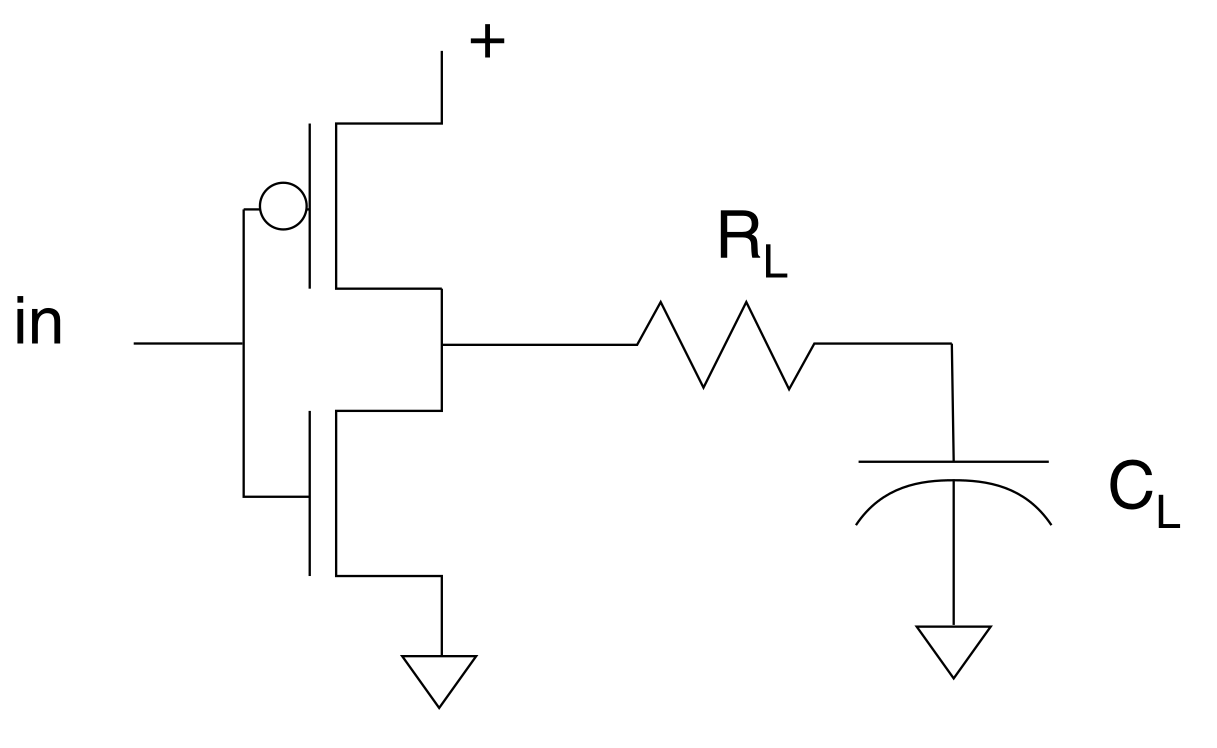
\includegraphics[width=0.7\linewidth]{Imagenes/02-Inversor_2.png}    
    \caption{modelización del retardo de puerta lógica inversora.}
    \label{Fig:02-Inversora_RC}
\end{figure}


El \textbf{modelo tau ($\boldsymbol{\tau}$)} nos da un valor para el retardo. Este modelo reduce el retardo de la puerta a un RC de tiempo constante $\tau$ para ambos modos. Que un transistor este modelado por una resistencia $R_n$ puede sonar un poco raro, y más cuando el transitor no obedece una ley lineal de entrada-salida (ley de Ohm). Por ello seleccionar una resistencia puede ser un poco complicado. Lo que se hace normalmente es asumir que la resistencia es un promedio del voltaje en saturacion y en el comporamiento lineal: 

\begin{equation}
    R_n = \frac{1}{2} \parentesis{\frac{V_{sat}}{I_{sat}}+\frac{V_{lin}}{I_{lin}}}
\end{equation}
Los valores de voltaje e intensidad de saturación y lineal dependerán del transistor. Además tenemos la \textit{resistencia de carga} (\textit{load resistance}), que es la resistencia efectiva que se conecta a la salida de un circuito. Es el elemento resistivo que determina cuánta corriente debe entregar el circuito para mantener un determinado voltaje en la salida.Esta resistencia de carga suele está conectada en serie con la resistencia $R_n$, por lo que la resistencia efectiva es: 

\begin{equation}
    R_{eff} = R_n + R_L
\end{equation} 
El tiempo de retardo vendrá dado por: 

\begin{equation}
    \tau \propto (R_n + R_L) C_L
\end{equation}
Otro modelo es el \textbf{modelo para una fuente de corriente}, el cual se suele usar en estudios de potencia-retardo. Si asumimos que el transistor actúa como una fuente de corriente cuyo $V_{gs}=V_g-V_s$\footnote{El $V_{gs}$ es el que controla que el canal este formado, por lo que si es menor que el umbral el transistor no estará encendido y si supera el umbral en transistor estará encendido.} está siempre al máximo valor, entonces el tiempo que tarda en decaer viene dado por 

\begin{equation}
    t_f = \frac{C_L (V_{DD}-V_{SS})}{I_d}
\end{equation}
Otro modelo es el \textbf{modelo ajustado}, que directamente lo que hace es medir experimentalmente las características del sistema y ajustarlas con una función que sea capaz de reproducirla. Suele ser usada en programas que analizan un gran número de puertas. 

Este análisis con RC nos arroja información sobre el retardo temporal. En primer lugar, que los retardos de 0 a 1 y de 1 a 0 serán diferentes (el 0 a 1 será más rápido, entorno a la mitad o un ternio de 1 a 0) debido a la diferencia del ratio de las resistencias efectivas. 

\subsection{Consumo de potencia}

En consumo de potencia es un punto importante cuando hablamos sobretodo de dispositivos en la vida real. El consumo en los circuitos CMOS depende directamente de la frecuencia en la que operen los aparatos, del tamaño de los transistores (sobretodo aquellos que tengan mayor influencia en la capacidad), así como de la diferencia de los voltajes $V_{DD}$ y $V_{SS}$ en los que opere el circuito, tal que la potencia $P$ es

\begin{equation}
    P = f C_L (V_{DD}-V_{SS})^2
\end{equation}
siendo $f$ la \textit{frecuencia de reloj} y $C_L$ la capacidad del sistema. En muchas ocasiones hablamos de la \textit{speed-power} a la périda de energía que ocurre en una sola transición, definida como el producto $SP=CV^2$. Como podemos ver, las pérdidas de energía se reducen cuando disminuimos el voltaje al que operamos, por eso se busca usar puertas lógicas en paralelo. Reducir el voltaje hace más lentos los transistores, por lo que tienes que disminuir la frecuencia si quieres bajar el voltaje. Ahoran, si necesitas procesar la misma cantidad de datos por segundo, agregas más unidades lógicas en paralelo, cada una trabajando más despacio (menor frecuencia) pero todas colaborando para mantener el rendimiento global. A esta técnica se le llama \textbf{escalado de voltaje}.

\subsection{Manejando grandes cargas}

\subsection{Puertas de baja potencia}

\subsection{\textit{Switch Logic}}


El símbolo mostrado en la  \cref{Fig:02-switch} representa un transistor de transmisión controlado por una señal de reloj o fase. También se le llama switch controlado o interruptor de transmisión.

La señal a en la parte superior indica la señal de control: cuando a está activa, el interruptor se cierra y conecta las dos líneas horizontales. La señal a' (a prima) representa la fase complementaria: a' es simplemente la inversión de a, aunque en el símbolo no siempre se conecta explícitamente; a menudo solo se indica que este interruptor trabaja con fases alternas.

Cuando a está en nivel alto (a=1), el interruptor cierra el contacto, permitiendo que la señal de la línea izquierda pase a la derecha y viceversa. Es decir, el interruptor está conduciendo. Cuando a está en nivel bajo (a=0), el interruptor se abre, aislando eléctricamente ambos lados; las señales no pueden pasar.

\begin{figure}[H] \centering
    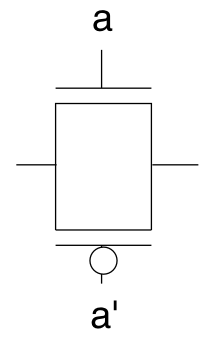
\includegraphics[width=0.3\linewidth]{Imagenes/02-Switch}
    \caption{Puerta de trasmisión complementaria.}
    \label{Fig:02-switch}
\end{figure}

¿Por  que hay dos transistores, un n-mos y un p-mos? Porque la conducción de n-mos depende de si el valor de entrada es 0 o 1, ya qeu conduce bien para 0 pero mal para 1. Con a y a' esto se soluciona: cuando a=1, el nMOS se enciende y a'=0, el pMOS también se enciende, ambos conducen y el paso es limpio en todo el rango de tensión. Cuando a=0, el nMOS se apaga y a'=1, el pMOS se apaga, ambos desconectados y el paso cortado.

\section{Cables}

\subsection{Estrcutra de los cables}

\subsection{Modelos de cables}


\section{Registros y RAM}

La memoria en sus difernetes formas es muy importante en el diseño digital y particularmente interesante en los FPGAs. En este sección vamos a hablar de los registros -elementos de memoria diseñados para hacer operaciones de reloj- y el acceso a memoria.  

En este contexto, un \textbf{reloj} es una señal eléctrica periódica que alterna entre niveles alto y bajo.  Cada transición de la señal de reloj se llama \textbf{flanco}. El \textbf{tiempo de setup} (setup time) es el tiempo mínimo que la señal de datos (D) debe estar estable antes del flanco activo del reloj (por ejemplo, el flanco de subida) para que el registro pueda capturarla correctamente. El \textbf{tiempo de hold} (hold time) es el tiempo mínimo que la señal de datos debe permanecer estable después del flanco activo del reloj, para asegurar que el registro complete la captura del dato.

Los \textbf{\textit{latches}} (biestable) son elementos de almacenamiento que guardan un bit y cuya salida sigue la entrada mientras la señal de habilitación está activa (nivel alto o bajo, según el diseño). Por eso se dice que son transparentes: mientras la habilitación esté activa, cualquier cambio en la entrada se refleja inmediatamente en la salida. Cuando la habilitación deja de estar activa, el latch mantiene el último valor capturado.

Los \textbf{flip-flop} también almacenan un bit, pero su salida solo se actualiza en el instante de un flanco del reloj (subida o bajada). Esto significa que los datos se capturan solo en un momento preciso definido por el reloj, no mientras un nivel esté activo. Por eso son la base de los registros sincrónicos en circuitos digitales.

\subsection{Estrucutra de los registros}

Construir una máquina secuencial requiere \textbf{registros} que lean un valor, lo guarden durante un tiempo, y que luego puedan escribir  el valor guardado en algún sitio, incluso si el valor de entrada cambia  para asegurar que la máquina secuencial opere correctamente paso a paso. Es decir, una vez que el registro captura un dato, ese dato queda “congelado” dentro del registro hasta que el reloj indique que debe capturar un nuevo valor. 


En los circuitos CMOS, la memoria de un registro se forma por algún tipo de capacitancia o mediante retroalimentación positiva de energía desde la fuente de alimentación. El acceso a la memoria interna se controla mediante la entrada de reloj: el elemento de memoria lee el valor de su entrada de datos cuando el reloj lo indica y almacena ese valor en su memoria. La salida refleja el valor almacenado, probablemente después de algún retardo. Los registros difieren en muchos aspectos clave:

\begin{itemize}
    \item La forma de la señal de reloj que imprime el valor de entrada en el registro. 
    \item Como el comportamiento de la información sobre la señal de lectrua de un reloj afecta al valor guardado. Ejemplo: Supón que el registro necesita un setup de 5 ns y un hold de 1 ns. Si el dato cambia 1 ns antes del flanco, se violó el setup, y entonces el valor almacenado puede ser incorrecto. Si el dato cambia 0.5 ns después del flanco, entonces se violó el hold, y también puede capturarse un valor erróneo.
    \item Cuando el valor guardado es presentado como un valor de salida . 
    \item Si alguna vez existe un camino combinacional desde la entrada hasta la salida. Se refiere a si, en un registro o máquina secuencial, hay una ruta directa de lógica combinacional que conecta la entrada con la salida sin intervención del registro (sin esperar al reloj). Si no existe (lo habitual en registros bien diseñados), la salida solo cambia cuando el reloj captura un nuevo valor.
\end{itemize}
La salida de un latch sigue su entrada mientras la entrada de reloj del latch está activa; en contraste, un flip-flop permite que la entrada afecte a la salida solo en una ventana muy estrecha alrededor de un flanco del reloj. ChatGPT Plus Los latches se usan en circuitos digitales cuando se necesita almacenar un bit de información con un control de nivel (en lugar de control por flanco), y permiten ciertas aplicaciones específicas donde su comportamiento de “transparencia” resulta útil. Por ejemplo, en interfaces de comunicación entre bloques que funcionan a diferentes velocidades.

El registro más simple de CMOS consiste en una \textbf{\textit{latch dinámica}}. Dinámica porque su valor de memoria no es refrescada por la fuente de alimentación y \textit{latch} porque su salida sigue a su entrada bajo algunas condiciones.  

\begin{figure}[H] \centering
    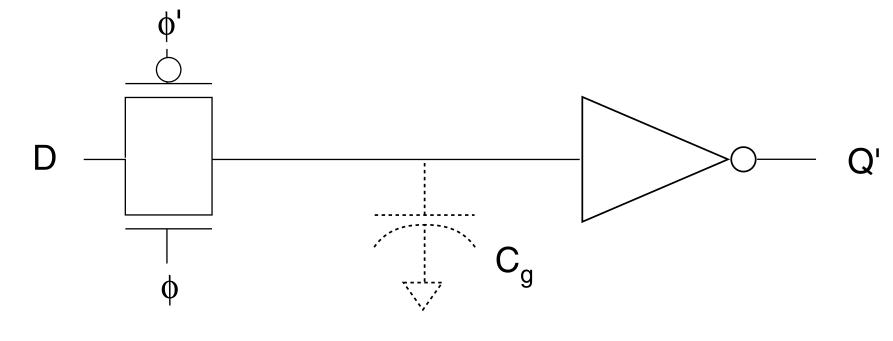
\includegraphics[width=0.7\linewidth]{Imagenes/02-LatchDinamica.png}
    \caption{un esquema de la latch-dinámica.}
    \label{Fig:02-LatchDinamica}
\end{figure}

El registro más simple en tecnología CMOS es el latch dinámico mostrado en la \cref{Fig:02-LatchDinamica}. Se le llama dinámico porque el valor almacenado en la memoria no se refresca mediante la fuente de alimentación, y se le llama latch porque su salida sigue a su entrada mientras está habilitado.



La entrada es D en un latch tipo D, por lo que su salida es Q’. El inversor conectado a la salida debería resultarte familiar. La capacitancia de almacenamiento se ha representado con líneas punteadas, ya que es un componente parasitario; esta capacitancia se ha denominado $C_g$ porque la mayor parte de ella proviene de las puertas de los transistores en el inversor.

El funcionamiento del latch es sencillo. Cuando el transistor de transmisión está encendido, cualquier puerta lógica conectada a la entrada D puede cargar o descargar $C_g$. A medida que el voltaje en $C_g$ cambia, Q’ sigue ese cambio de forma complementaria: cuando $C_g$ se lleva a voltajes bajos, Q’ sube a voltajes altos, y viceversa. Cuando el transistor de transmisión se abre, $C_g$ queda desconectado de cualquier puerta lógica que pudiera cambiar su valor. Por lo tanto, el valor de la salida Q’ del latch depende del voltaje del condensador de almacenamiento: si el condensador se ha descargado, la salida del latch será un 1 lógico; si el condensador se ha cargado, la salida del latch será un 0 lógico. Es importante notar que el valor de Q’ es el complemento lógico del valor presentado al latch en D; debemos tener en cuenta esta inversión al usar el latch. Para cambiar el valor almacenado en el latch, podemos cerrar el transistor de transmisión estableciendo $\phi = 1$ y $\phi’ = 0$, y luego cambiar el voltaje en $C_g$.

\begin{figure}[H] \centering
    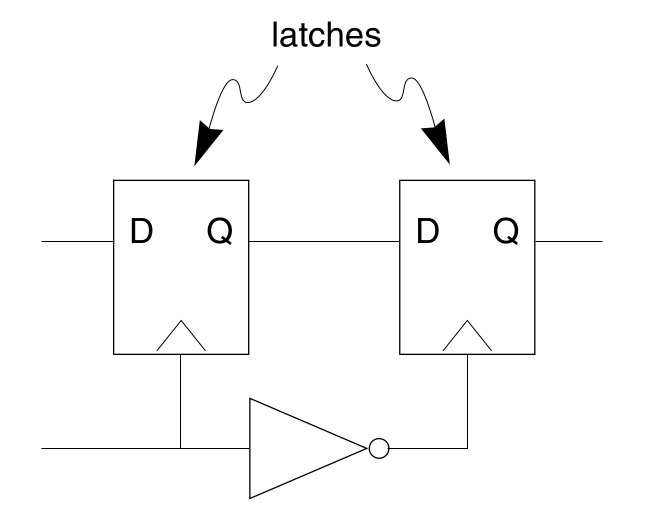
\includegraphics[width=0.6\linewidth]{Imagenes/02-FlipFlop.png}
    \caption{un flip-flop hecho de latches.}
    \label{Fig:02-FlipFlop}
\end{figure}

La estructura de un flip-flop activado por flanco se muestra en la \cref{Fig:02-FlipFlop}. Se construye a partir de dos latches conectados en cascada. El primer latch lee la entrada de datos cuando el reloj está en alto. Mientras tanto, el inversor interno asegura que la entrada de reloj del segundo latch esté en bajo, aislando al segundo latch de los cambios en la salida del primer latch y manteniendo estable el valor de salida del flip-flop. Después de que el reloj pasa a nivel bajo, la entrada de reloj del segundo latch queda en alto, haciéndolo transparente, pero el primer latch presenta un valor estable al segundo latch. Cuando el reloj vuelve de 0 a 1, el segundo latch guarda su valor antes de que la salida del primer latch tenga oportunidad de cambiar.



\chapter{Estrcuturas de sistemas FPGA}







\end{document}